\documentclass{ximera}
\title[Examples:]{Graphics and videos}
\author{Sara Malec \and Jack Schmidt \and Bart Snapp}

\begin{document}
\begin{abstract}
Instructions for making graphics and videos.
\end{abstract}
\maketitle

\section{Images}
One way to insert images into a Ximera activity, is to have the image
in the directory with \verb|\includegraphics|.  We recommend using the
\verb|image| environment for all of you images.
\begin{verbatim}
\begin{image}
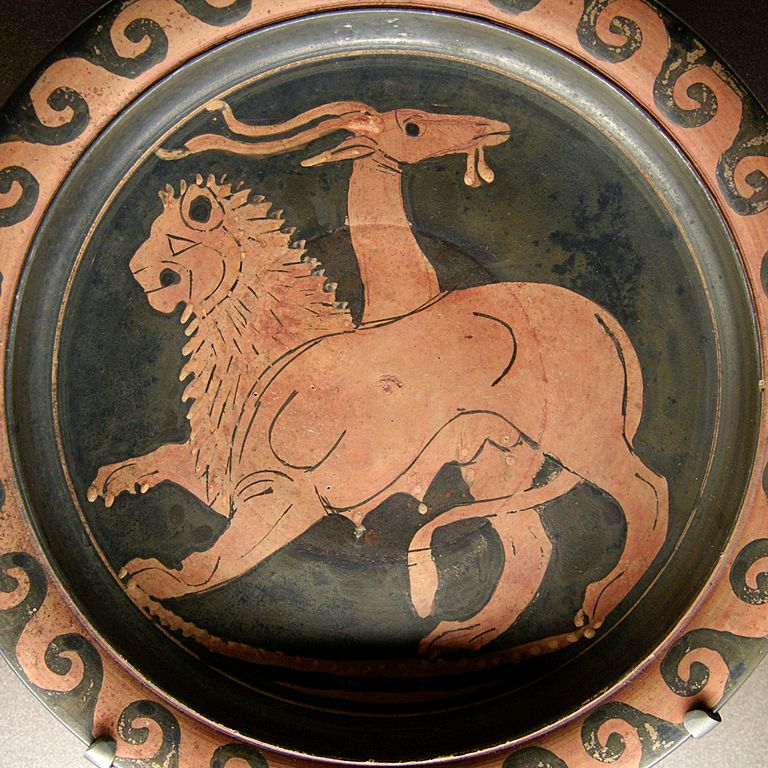
\includegraphics{chimera.jpg}
\end{image}
\end{verbatim}
\begin{image}
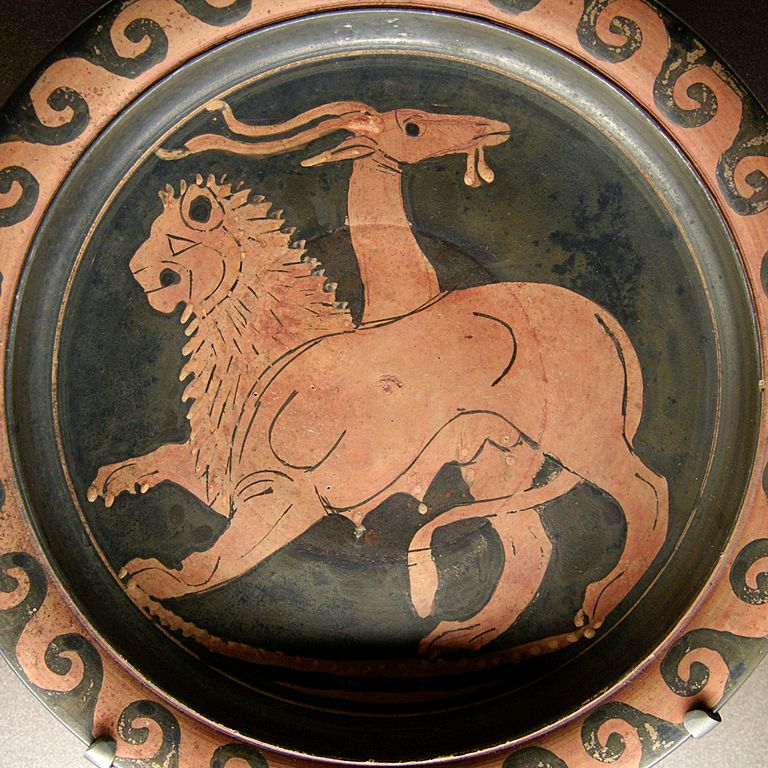
\includegraphics{chimera.jpg}
\end{image}
Note, you may need to update your graphics path in the xourse file, so
that the xourse file can find your graphic. This can be set up in the
preamble like this:
\begin{verbatim}
\graphicspath{
{./}
{graphicsAndVideos/}
}
\end{verbatim}

To add graphics side-by-side, you can just place them in \verb|image| tags:

\begin{center}
  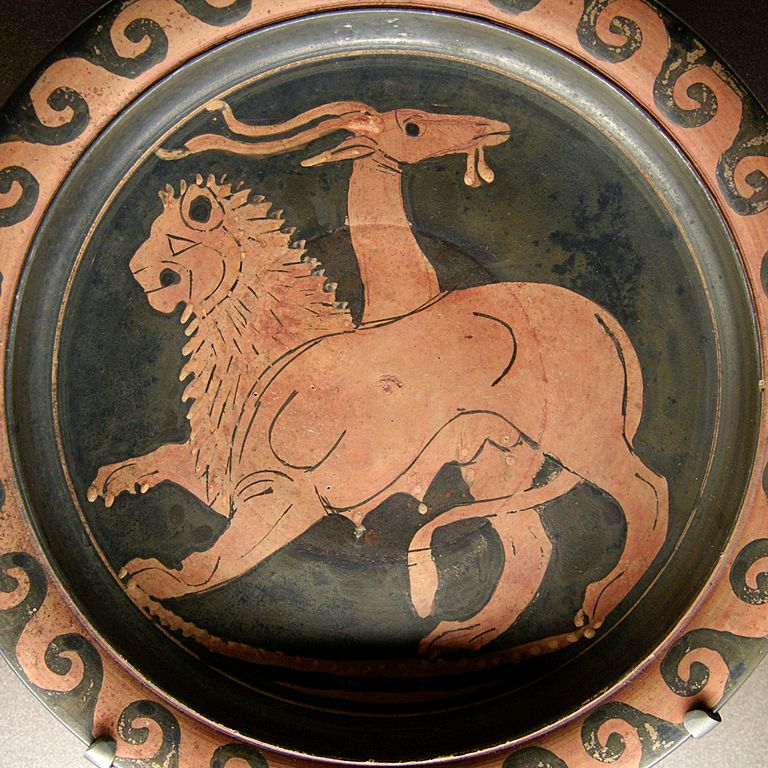
\includegraphics{chimera.jpg}\quad
  
\includegraphics{dna.jpg}
\end{center}
\begin{verbatim}
\begin{center}
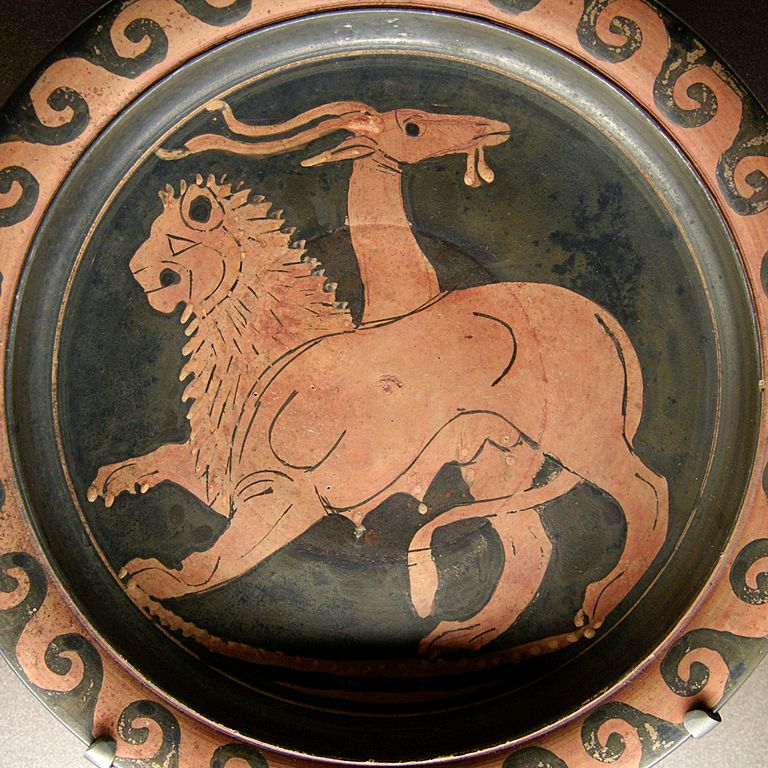
\includegraphics{chimera.jpg}\quad

\includegraphics{dna.jpg}
\end{center}
\end{verbatim}
When done this way, the pictures will rearrange themselves depending on the width of the screen.



Another way to include graphics is to use Tikz. In some sense this is
preferred, as then the source produces the images.
\begin{image}
  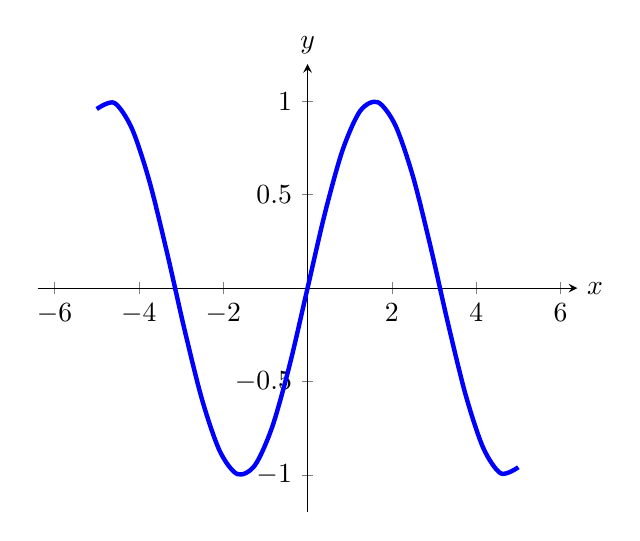
\begin{tikzpicture}
    \begin{axis}[
        xmin=-6.4,
        xmax=6.4,
        ymin=-1.2,
        ymax=1.2,
        axis lines=center,
        xlabel=$x$,
        ylabel=$y$,
        every axis y label/.style={at=(current axis.above origin),anchor=south},
        every axis x label/.style={at=(current axis.right of origin),anchor=west},
      ]
      \addplot [ultra thick, blue, smooth] {sin(deg(x))};
    \end{axis}
  \end{tikzpicture}
\end{image}

\begin{verbatim}
\begin{image}
  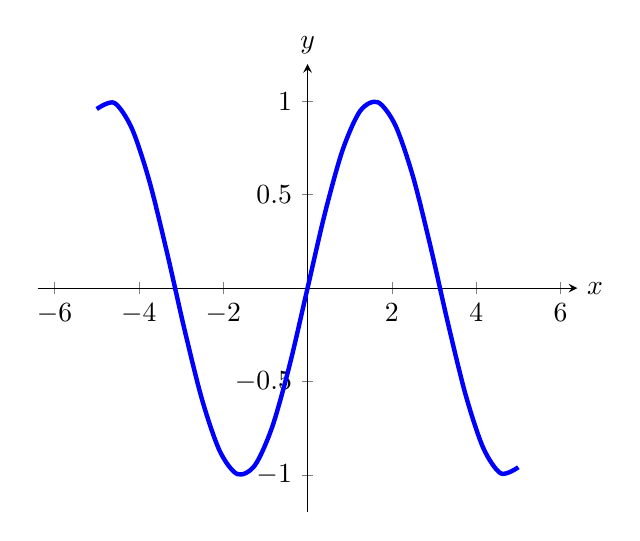
\begin{tikzpicture}
    \begin{axis}[
        xmin=-6.4,
        xmax=6.4,
        ymin=-1.2,
        ymax=1.2,
        axis lines=center,
        xlabel=$x$,
        ylabel=$y$,
        every axis y label/.style={at=(current axis.above origin),anchor=south},
        every axis x label/.style={at=(current axis.right of origin),anchor=west},
      ]
      \addplot [ultra thick, blue, smooth] {sin(deg(x))};
    \end{axis}
  \end{tikzpicture}
\end{image}
\end{verbatim}



\section{Interactive graphics}


\subsection{The graph command}

The easiest way to include an interactive graph is to use the
\verb|\graph| command. Unfortunately, the \verb|\graph| command
doesn't draw a graph in the PDF, rather, it states (in words) that a
graph is produced.
\[
\graph{x^2}
\]
There are a number of options for the \verb|\graph| command:


\paragraph{Change viewing window}

  
\begin{verbatim}
\[
\graph[xmin=-5,xmax=5,ymin=-5,ymax=5]{y=x^2}
\]
\end{verbatim}
\paragraph{Restricting domain}


\begin{verbatim}
\[
\graph{x^2 \left\{ 1 \leq x \leq 10 \right\} }
\]
\end{verbatim}
\paragraph{Default panel displayed}

  
\begin{verbatim}
\[
\graph[panel]{x^2}
\]
\end{verbatim}
\paragraph{Restricting window}

  
\begin{verbatim}
\[
\graph[xmin=0, xmax=10, ymin=0, ymax=10]{x^2}
\]
\end{verbatim}
\paragraph{Axis labels}

  
\begin{verbatim}
\[
\graph[xAxisLabel="time", yAxisLabel="distance"]{y=x}
\]
\end{verbatim}
\paragraph{Hide axes}

  
\begin{verbatim}
\[
\graph[hideXAxis=true, hideYAxis=true]{x^2}
\]
\end{verbatim}
\paragraph{Hide tick marks}

  
\begin{verbatim}
\[
\graph[hideXAxisNumbers=true, hideYAxisNumbers=true]{x=y^2}
\]
\end{verbatim}
\paragraph{Polar graphing}

  
\begin{verbatim}
\[
\graph{r=\theta}
\]
\end{verbatim}
\paragraph{Polar gridlines}


\begin{verbatim}
\[
\graph[polar]{y=x^2}
\]
\end{verbatim}
\paragraph{Graphing a piecewise function}


\begin{verbatim}
\[
\graph{ \sin(x)\left\{x<0\right\}, 2x\left\{ x>=0 \right\} }
\]
\end{verbatim}


\subsection{Desmos}

If you require further features from
\link[Desmos]{https://www.desmos.com/}, you can sign up for an account
and include your worksheets like this:

\begin{verbatim}
\begin{center}
\desmos{zwywds7med}{800}{600}
\end{center}
\end{verbatim}
\begin{center}
\desmos{zwywds7med}{800}{600}
\end{center}


\subsection{GeoGebra}

You can also use \link[GeoGebra]{https://www.geogebra.org/}. Embed the
widget using the syntax \verb|\geogebra{ID}{width}{height}|, where ID
is the widget ID and width and height are the dimensions (in pixels)
you want the embedded widget to have.
\begin{center}
  \geogebra{XC3FXUdJ}{800}{600}%%https://www.geogebra.org/m/XC3FXUdJ
\end{center}

\begin{verbatim}
\begin{center}
\geogebra{XC3FXUdJ}{800}{600}
\end{center}
\end{verbatim}

Note, you may wish to use the \verb|onlineOnly| environment with your
interactives.

\section{Videos}

You can also embed \link[YouTube]{https://www.youtube.com/} videos.
\begin{center}
\youtube{0aQpLSu2fMs}
\end{center}

\begin{verbatim}
\begin{center}
\youtube{0aQpLSu2fMs}
\end{center}
\end{verbatim}


\end{document}
